\documentclass[10pt]{article}
\usepackage[margin=2cm]{geometry}
\usepackage{booktabs,graphicx,amsmath,amssymb,xcolor}
% generated by make_report.py -- do not edit
\newcommand{\RAEmerkitDfr}{3.3}
\newcommand{\RAEmerkitEq}{69.8}
\newcommand{\RAEmerkitQviol}{0.2}
\newcommand{\RAEmerkitRed}{0.09}
\newcommand{\RAEmerkitValid}{67.3}
\newcommand{\RAEmerkitXiDfr}{6.5}
\newcommand{\RAEmerkitXiEq}{76.1}
\newcommand{\RAEmerkitXiQviol}{0.2}
\newcommand{\RAEmerkitXiRed}{0.08}
\newcommand{\RAEmerkitXiValid}{71.1}
\newcommand{\RAEmkCpMax}{0.0}
\newcommand{\RAEmkNoIntCpMax}{0.4}
\newcommand{\RAOracleDfr}{0.0}
\newcommand{\RAOracleEq}{78.9}
\newcommand{\RAOracleQviol}{0.2}
\newcommand{\RAOracleRed}{0.07}
\newcommand{\RAOracleValid}{78.7}
\newcommand{\RAOverEmk}{7.8}
\newcommand{\RAOverNoInt}{15.6}
\newcommand{\RAOverRag}{53.8}
\newcommand{\RAOverZeng}{11.8}
\newcommand{\RARagCpMax}{54.7}
\newcommand{\RARagExceed}{99.2}
\newcommand{\RARagMcpDfr}{78.9}
\newcommand{\RARagMcpEq}{100.0}
\newcommand{\RARagMcpPlusFilterDfr}{20.5}
\newcommand{\RARagMcpPlusFilterEq}{100.0}
\newcommand{\RARagMcpPlusFilterQviol}{30.1}
\newcommand{\RARagMcpPlusFilterRed}{1.79}
\newcommand{\RARagMcpPlusFilterValid}{31.3}
\newcommand{\RARagMcpQviol}{55.6}
\newcommand{\RARagMcpRed}{2.25}
\newcommand{\RARagMcpValid}{8.1}
\newcommand{\RAZengDfr}{45.2}
\newcommand{\RAZengEq}{99.5}
\newcommand{\RAZengExceed}{56.8}
\newcommand{\RAZengPlusFilterDfr}{11.5}
\newcommand{\RAZengPlusFilterEq}{82.0}
\newcommand{\RAZengPlusFilterQviol}{0.1}
\newcommand{\RAZengPlusFilterRed}{0.04}
\newcommand{\RAZengPlusFilterValid}{72.6}
\newcommand{\RAZengQviol}{0.6}
\newcommand{\RAZengRed}{0.07}
\newcommand{\RAZengValid}{54.5}
\newcommand{\RBAmbEpsZeroFive}{10.9}
\newcommand{\RBDfrThree}{3.2}
\newcommand{\RBEpsThree}{0.070}
\newcommand{\RBEqEpsZero}{22.7}
\newcommand{\RBEqHigh}{77.9}
\newcommand{\RBEqHundred}{26.1}
\newcommand{\RBEqLow}{26.1}
\newcommand{\RBEqThree}{69.8}
\newcommand{\RBMaxDfrRatio}{0.69}
\newcommand{\RCapPrec}{100.0}
\newcommand{\RCapRec}{96.6}
\newcommand{\RConfCovFive}{95.9}
\newcommand{\RConfCovTen}{92.7}
\newcommand{\RConfCovTwenty}{91.5}
\newcommand{\RDAdditiveUtilityDfr}{4.5}
\newcommand{\RDAdditiveUtilityEq}{69.8}
\newcommand{\RDAdditiveUtilityQviol}{0.0}
\newcommand{\RDAdditiveUtilityRed}{1.10}
\newcommand{\RDDeclaredAnnotationsDfr}{19.0}
\newcommand{\RDDeclaredAnnotationsEq}{80.9}
\newcommand{\RDDeclaredAnnotationsQviol}{0.2}
\newcommand{\RDDeclaredAnnotationsRed}{0.08}
\newcommand{\RDFullEmerkitDfr}{3.3}
\newcommand{\RDFullEmerkitEq}{69.8}
\newcommand{\RDFullEmerkitQviol}{0.2}
\newcommand{\RDFullEmerkitRed}{0.09}
\newcommand{\RDNoInteractionsDfr}{3.3}
\newcommand{\RDNoInteractionsEq}{69.8}
\newcommand{\RDNoInteractionsQviol}{0.2}
\newcommand{\RDNoInteractionsRed}{0.14}
\newcommand{\RDNoQosDfr}{4.1}
\newcommand{\RDNoQosEq}{76.5}
\newcommand{\RDNoQosQviol}{46.1}
\newcommand{\RDNoQosRed}{0.23}
\newcommand{\RLabAccMax}{95.9}
\newcommand{\RLabAccMin}{85.7}
\newcommand{\RNSeeds}{5}
\newcommand{\RNTasks}{1500}
% generated by make_report2.py
\newcommand{\RAfourEmk}{82.2}
\newcommand{\RAfourEmkSevenFive}{11.1}
\newcommand{\RAfourRag}{8.4}
\newcommand{\RAfourZeng}{60.9}
\newcommand{\RAfourZengSevenFive}{10.0}
\newcommand{\RAuAgree}{26}
\newcommand{\RAuLowConf}{5}
\newcommand{\RAuOut}{24}
\newcommand{\RAuReviewed}{40}
\newcommand{\RAuServers}{40}
\newcommand{\RAuTools}{210}
\newcommand{\RBthreeDeclMax}{16.7}
\newcommand{\RBthreeEmkMax}{3.3}
\newcommand{\RBthreeZengHigh}{15.6}
\newcommand{\RBtwoDeclMeight}{18.2}
\newcommand{\RBtwoDeclMzero}{3.4}
\newcommand{\RBtwoEmkMax}{5.7}
\newcommand{\RBtwoEmkMin}{3.3}
\newcommand{\RBtwoEqWtwenty}{67.8}
\newcommand{\RBtwoEqWzero}{87.3}
\newcommand{\RBtwoRagMax}{21.8}
\newcommand{\RBtwoZengMax}{14.8}
\newcommand{\RCfourEmkLarge}{8}
\newcommand{\RCfourEmkSmall}{7}
\newcommand{\RCfourMem}{270}
\newcommand{\RCfourPrep}{1.00}
\newcommand{\RCfourReal}{0.3}
\newcommand{\RCthreeConf}{2.3}
\newcommand{\RCthreeInfFive}{85.9}
\newcommand{\RCthreeMedMax}{0.16}
\newcommand{\RCthreePmax}{0.31}
\newcommand{\RCthreeTo}{0.0}
\newcommand{\RCtwoAllCons}{79.2}
\newcommand{\RCtwoAllThree}{84.7}
\newcommand{\RCtwoAllTwo}{83.3}
\newcommand{\RCtwoAllZero}{55.6}
\newcommand{\RCtwoNoWf}{0.0}
\newcommand{\RCtwoObjMin}{99.3}
\newcommand{\RCtwoPrereq}{0}
\newcommand{\RCtwoPres}{0}
\newcommand{\RCtwoRagRisk}{100.0}
\newcommand{\RCtwoSub}{9.7}
\newcommand{\RCtwoTaskDfr}{6.9}
\newcommand{\RCtwoWfRisk}{34.7}
\newcommand{\RCtwoWfRiskCons}{37.5}
\newcommand{\RCtwoZAll}{93.1}
\newcommand{\RCtwoZRisk}{91.7}
\newcommand{\RCtwoZfAll}{56.9}
\newcommand{\RCtwoZfRisk}{36.1}
\newcommand{\RDtwoRedI}{0.07}
\newcommand{\RDtwoRedNoI}{0.14}
\newcommand{\RDtwoValidMax}{83.6}
\newcommand{\RDtwoValidMin}{82.2}
\newcommand{\REoneRiskStd}{7.1}
\newcommand{\REoneRiskStrict}{11.2}
\newcommand{\REoneSafeSyn}{89.1}
\newcommand{\REoneUncMix}{13.1}
\newcommand{\REoneUncSyn}{3.8}
\newcommand{\REtwoUncHalf}{1.3}
\newcommand{\RFoneBlocked}{100.0}
\newcommand{\RFoneDenied}{2.8}
\newcommand{\RFoneExact}{100.0}
\newcommand{\RFoneExposed}{100.0}
\newcommand{\RFoneN}{72}
\newcommand{\RFoneSec}{1.3}
\newcommand{\RFoneSeeds}{3}
% generated by make_report3.py
\newcommand{\RAfiveAucBase}{0.52}
\newcommand{\RAfiveAucConf}{0.73}
\newcommand{\RAfiveAucSim}{0.82}
\newcommand{\RAfiveCoefConf}{-3.42}
\newcommand{\RAfiveCoefLoad}{0.03}
\newcommand{\RAfiveCoefSat}{0.007}
\newcommand{\RAfiveCoefSim}{-0.91}
\newcommand{\RAfiveHaikuConf}{84.8}
\newcommand{\RAfiveHaikuRand}{99.2}
\newcommand{\RAfiveModels}{2}
\newcommand{\RAfiveN}{1000}
\newcommand{\RAfiveOpusConf}{81.6}
\newcommand{\RAfiveOpusRand}{99.6}
\newcommand{\RAfivePConf}{< 0.001}
\newcommand{\RAfivePLoad}{0.91}
\newcommand{\RAfivePSat}{0.022}
\newcommand{\RAfiveSyn}{98.2}
\newcommand{\RAuHaikuAgree}{19}
\newcommand{\RAuHaikuDec}{168}
\newcommand{\RAuHaikuN}{34}
\newcommand{\RAuPair}{152}
\newcommand{\RAuPairN}{168}
\newcommand{\RAuSonnetAgree}{30}
\newcommand{\RAuSonnetDec}{209}
\newcommand{\RAuSonnetN}{40}
\newcommand{\RCoCpEq}{100.0}
\newcommand{\RCoCpObj}{70.8}
\newcommand{\RCoCpRisk}{100.0}
\newcommand{\RCoLgEq}{84.8}
\newcommand{\RCoLgObj}{100.0}
\newcommand{\RCoLgPrereq}{0}
\newcommand{\RCoLgRaw}{91.7}
\newcommand{\RCoLgRisk}{13.3}
\newcommand{\RCoLgValid}{83.3}
\newcommand{\RCoN}{72}
\newcommand{\RCoSeeds}{3}
\newcommand{\RFlBlocked}{100.0}
\newcommand{\RFlDenied}{0}
\newcommand{\RFlExposed}{100.0}
\newcommand{\RFlN}{27}
\newcommand{\RFlRealised}{22.1}
\newcommand{\RFlSeeds}{3}
\newcommand{\RFlUnexp}{0}
\newcommand{\RJfCorr}{0.67}
\newcommand{\RJfGap}{0.23}
\newcommand{\RJfInter}{0.85}
\newcommand{\RJnAgree}{93.5}
\newcommand{\RJnDis}{7}
\newcommand{\RJnItems}{108}
\newcommand{\RJnKappa}{1.00}
\newcommand{\RJsAgree}{73.7}
\newcommand{\RJsDis}{5}
\newcommand{\RJsItems}{19}
\newcommand{\RJsKappa}{0.91}
\newcommand{\RLaMapRec}{95.9}
\newcommand{\RLaPrec}{100.0}
\newcommand{\RLaRec}{97.1}
\newcommand{\RPonePanelDfr}{2.4}
\newcommand{\RPonePanelEq}{83.6}
\newcommand{\RPonePanelZfDfr}{7.4}
\newcommand{\RPoneStandardDfr}{3.4}
\newcommand{\RPoneStandardEq}{85.3}
\newcommand{\RPoneStandardZfDfr}{4.8}
\newcommand{\RPtwoPanelAll}{81.9}
\newcommand{\RPtwoPanelRisk}{30.6}
\newcommand{\RPtwoPanelSub}{14.1}
\newcommand{\RPtwoStandardAll}{83.3}
\newcommand{\RPtwoStandardRisk}{34.7}
\newcommand{\RPtwoStandardSub}{9.7}
\newcommand{\RSixEmk}{73.8}
\newcommand{\RSixEmkAvail}{77.6}
\newcommand{\RSixEmkClones}{0.68}
\newcommand{\RSixN}{500}
\newcommand{\RSixP}{0.25}
\newcommand{\RSixRag}{73.0}
\newcommand{\RSixRagAvail}{76.6}
\newcommand{\RSixRagClones}{1.67}
\newcommand{\RSixRnd}{42.2}
\newcommand{\RSixRndAvail}{43.6}
\newcommand{\RSixRndClones}{1.08}
% generated by make_report4.py
\newcommand{\RClHaiku}{93.6}
\newcommand{\RClOpus}{95.2}
\newcommand{\RClShare}{66.7}
\newcommand{\RFitAuc}{0.83}
\newcommand{\RFitAucBase}{0.52}
\newcommand{\RFitLamC}{-0.003}
\newcommand{\RSvColdN}{200}
\newcommand{\RSvColdNoTraces}{3.8}
\newcommand{\RSvColdRag}{12.0}
\newcommand{\RSvColdTraces}{1.8}
\newcommand{\RSvColdZeng}{0.0}
\newcommand{\RSvSuccess}{2,218}
\newcommand{\RSvTools}{766}
\newcommand{\RSvTraces}{3,500}
\newcommand{\RSvWarmN}{200}
\newcommand{\RSvWarmNoTraces}{5.0}
\newcommand{\RSvWarmRag}{19.3}
\newcommand{\RSvWarmTraces}{9.3}
\newcommand{\RSvWarmZeng}{0.4}
\newcommand{\RWcSeeds}{3}
\newcommand{\RWcTaskAll}{72.2}
\newcommand{\RWcTaskEq}{96.0}
\newcommand{\RWcTaskRisk}{11.1}
\newcommand{\RWcWfAll}{0.2}
\newcommand{\RWcWfEq}{48.8}
\newcommand{\RWcWfRisk}{0.0}
% generated by make_paper_tables.py
\newcommand{\RXfiveExFifty}{90.0}
\newcommand{\RXfiveExMs}{190}
\newcommand{\RXfiveGrFifty}{77.4}
\newcommand{\RXfiveGrMs}{1.6}
\newcommand{\RXfiveLoss}{12.6}
\newcommand{\RXfiveRatio}{0.996}
\newcommand{\RXfourEmkRiskTen}{23.3}
\newcommand{\RXfourEmkRiskThree}{6.7}
\newcommand{\RXfourEmkTen}{65.0}
\newcommand{\RXfourEmkThree}{86.7}
\newcommand{\RXfourNsTen}{25.8}
\newcommand{\RXfourZRiskTen}{95.0}
\newcommand{\RXfourZTen}{92.5}
\newcommand{\RXfourZfRiskTen}{35.8}
\newcommand{\RXfourZfTen}{57.5}
\newcommand{\RXoneEmkDfrMax}{4.0}
\newcommand{\RXoneEmkMs}{25}
\newcommand{\RXoneEmkValidMax}{83.9}
\newcommand{\RXoneEmkValidMin}{22.8}
\newcommand{\RXoneMax}{630}
\newcommand{\RXoneMin}{60}
\newcommand{\RXoneZMs}{4}
\newcommand{\RXoneZfDfrMax}{15.1}
\newcommand{\RXoneZfValidMax}{93.9}
\newcommand{\RXsixAssessDfr}{10.9}
\newcommand{\RXsixDomMax}{2.9}
\newcommand{\RXsixLowDfr}{0.0}
\newcommand{\RXsixLowEq}{21.0}
\newcommand{\RXsixMatchDfr}{1.5}
\newcommand{\RXsixMatchEq}{67.3}
\newcommand{\RXtwoEmkDfrMax}{10.4}
\newcommand{\RXtwoEmkFive}{49.2}
\newcommand{\RXtwoEmkOne}{64.4}
\newcommand{\RXtwoOraFive}{53.6}
\newcommand{\RXtwoRagFive}{0.6}
\newcommand{\RXtwoZfDfrFive}{18.1}
\newcommand{\RXtwoZfFive}{70.0}

\newcommand{\sysname}{EmerKit}
\title{EmerKit: complete experimental results\\\large All experiments, tables, and figures, generated from the result files}
\date{}
\begin{document}
\maketitle
\noindent This document gathers every experimental result of EmerKit. Every number, table, and figure is generated from the result files of the repository (\texttt{make\_report*.py}, \texttt{make\_figures.py}, \texttt{make\_paper\_tables.py}); none is typed by hand. Part~I follows the organisation of the paper. Part~II gives the detailed tables of each series, named as in the repository: A0 and B0 (preparation), A1 (reference comparison), A2 to A4 (structure of toolkits, QoS bounds), A5 to A7 (probes, agent, trajectories), B1 to B3 (calibration, metadata, norms), C1 to C4 (end-to-end, solver, catalogue), D1 and D2 (ablations, weights), E1 and E2 (gap map), F1 (live enactment), P1 and P2 (model panel), and X1 to X6 (catalogue size, capabilities per task, workflow length, exact or greedy composition, distribution shift). Figures are also provided as vector PDF and 300-dpi PNG files.

\part*{Part I: Results}
\section{Implementation}\label{sec:impl}

\sysname{} is implemented in Python and consists of six components. The catalogue preparation component (Algorithm 1) extracts capabilities, infers behavioural labels by weak supervision and logistic regression, builds split-conformal prediction sets, and computes the interference index. The workflow generator is either rule-based or a language model, and a deterministic repair step followed by the validator enforces the contract of the paper. The composer (Algorithm 2) solves the composition program exactly with CP-SAT and explains infeasibility by a minimal conflict. The reviser (Algorithm 3) applies backtracking and substitution. The runtime executes every synthetic server as a real MCP server built with the official SDK, whose tools return learner data marked with canaries and actually forward what they receive, behind a gateway that exposes only the toolkit of the current task. Finally, the calibrator implements Learn-then-Test at the task level and at the workflow level. Ten property tests check the implementation against the definitions and propositions of the paper, including the equivalence between the constraints and the flow model, the optimality of the composer against exhaustive enumeration, and the minimality of conflicts. The language models are Claude Haiku~5.5, Sonnet~5.5, and Opus~5.5, and every call is logged.

\section{Experimental Protocol}\label{sec:setup}

\paragraph{Catalogues.} The experiments rely on two kinds of catalogues. The synthetic catalogue of educational MCP servers is regenerated for each seed, with about 165 tools on 36 servers, and it has a complete ground truth: capabilities, learner data returned, forwarding behaviour, receiver role, and near-duplicate pairs. Its observable side is deliberately noisy, since 60\% of the behavioural annotations are missing, 5\% of the present ones are wrong, and cues about data handling appear in 40\% of the descriptions. The real catalogues are MCP-tools, with 2{,}797 tools of 308 servers, and the Toucan server catalogue, with 6{,}044 tools described by full schemas, published annotations, categories, and measured success rates. We also use \RSvTraces{} Toucan trajectories, of which \RSvSuccess{} succeeded and call \RSvTools{} distinct tools.

\paragraph{Tasks and requests.} Tasks are generated independently of any scenario in three domains: data science, from the prerequisite graph of LectureBank~2.0; programming, from the Software Development Fundamentals area of CS2023; and English as a foreign language, from the CEFR progression. Each seed yields 300 test tasks, 50 per pedagogical type, 300 calibration tasks, and 24 learner requests for the end-to-end experiments.

\paragraph{Measures.} A task is \emph{equipped} when a toolkit is returned for it. A toolkit is \emph{valid} when it covers every required capability, allows no denied flow under the true labels, and meets the QoS bounds. The \emph{denied-flow rate} (DFR) is the share of returned toolkits that allow at least one denied flow. Redundancy is the number of providers beyond one per capability, and the load is the share of the budget $B$ used by the tool definitions. For workflows, we report the share that is fully equipped, the share that contains at least one risky toolkit, and the share of target concepts covered. The reference comparison uses five seeds and \RNTasks{} tasks; the other experiments use three seeds and the fixed level $\epsilon=0.05$ unless stated otherwise. Paired comparisons use Wilcoxon signed-rank tests with Holm correction.

\section{Compared Methods}\label{sec:methods}

Table~\ref{tab:methods} summarises the compared methods. RAG-MCP keeps the $k$ tools most similar to the task. QoS-IP denotes QoS-aware composition by integer programming, which selects one service per capability under global QoS constraints. Compositio Prompto (CP) asks a language model for the whole composition, given the service specifications, the task, and the output schema. Since no baseline handles norms, RAG-MCP and QoS-IP are also run with a filter that removes the tools whose declared annotations make a denied flow possible; these variants are denoted RAG-MCP+F and QoS-IP+F. The Oracle is \sysname{} supplied with the true labels, an upper bound that no deployable method can reach. Four variants of \sysname{} isolate its components: \sysname{}-NS disables substitution, \sysname{}-NI removes the interaction terms, \sysname{}-DA replaces the prediction sets by declared annotations, and \sysname{}-LLM places \sysname{} behind a language-model workflow generator.

\begin{table}[!ht]\centering
\caption{Compared methods and the aspects each one handles.}\label{tab:methods}
\scriptsize\setlength{\tabcolsep}{3pt}
\begin{tabular}{lcccccc}\toprule
Method & \rotatebox{70}{Capability once} & \rotatebox{70}{QoS bounds} & \rotatebox{70}{Interactions} & \rotatebox{70}{Flow norms} & \rotatebox{70}{Uncertain labels} & \rotatebox{70}{Workflow revision} \\ \midrule
RAG-MCP & -- & -- & -- & -- & -- & -- \\
RAG-MCP+F & -- & -- & -- & declared & -- & -- \\
QoS-IP & \checkmark & \checkmark & -- & -- & -- & -- \\
QoS-IP+F & \checkmark & \checkmark & -- & declared & -- & -- \\
CP & -- & -- & -- & -- & -- & -- \\
\sysname{} & \checkmark & \checkmark & \checkmark & \checkmark & \checkmark & \checkmark \\ \bottomrule
\end{tabular}\end{table}

\section{Parameter Settings and Experimental Design}\label{sec:params}

Table~\ref{tab:params} lists the parameters with their default values and the ranges explored. The interaction weights $\lambda_I$ and $\lambda_C$ are provisional defaults: the selection probes of Sect.~\ref{sec:res-h1} estimate them, and the sensitivity analysis of Sect.~\ref{sec:res-sens} shows that the results do not depend on them. Table~\ref{tab:series} gives an overview of the experiments, the research question that each one addresses, and the data that it uses.

\begin{table}[!ht]\centering
\caption{Parameter settings: defaults and values explored.}\label{tab:params}
\scriptsize\setlength{\tabcolsep}{3pt}
\begin{tabular}{llll}\toprule
Symbol & Meaning & Default & Explored \\ \midrule
$|\mathcal{T}|$ & tools in the catalogue & 165 & 60--2{,}960 \\
$|R(v)|$ & capabilities required per task & 1--4 & 1--5 \\
$|V|$ & tasks per workflow & 3--8 & 3--10 \\
$B$ & context budget (tokens) & 2{,}000 & 500--4{,}000 \\
$\theta$ & soft threshold of saturation & 0.75 & 0.5--0.9 \\
$k_{\max}$ & maximal toolkit size & 4 & 3--8 \\
$N$ & shortlist bound & 20 & 10--100 \\
$\tau$ & tightness of QoS bounds & 1.25 & 0.5--1.5 \\
$\lambda_I,\lambda_C$ & interaction weights & 1,\,1 & 0--2 \\
$\lambda_Q$ & weight of QoS deficit & 0.5 & 0--1 \\
$\eta$ & weight of trace evidence & 0.25 & 0,\,1 \\
$\xi,\zeta$ & target risk, confidence & 0.05,\,0.1 & $\xi$: 0.05--0.20 \\
$n_{cal}$ & calibration tasks & 300 & 45--300 \\
$\epsilon$ & level grid & 0--0.5 & 27 levels \\
$s_{\max}$ & substitutions per workflow & 2 & 0--3 \\
$n_W,\mu,\nu$ & candidates, penalties & 3,\,1,\,0.5 & $\nu$: 0.1--1 \\
$m,w$ & missing, wrong annotations & 0.6,\,0.05 & 0--0.8,\,0--0.2 \\ \bottomrule
\end{tabular}\end{table}

\begin{table}[!ht]\centering
\caption{Overview of the experiments.}\label{tab:series}
\scriptsize
\resizebox{\textwidth}{!}{\begin{tabular}{llcll}\toprule
Experiment & Question addressed & RQ & Catalogue & Scale \\ \midrule
Selection probes & Do co-present tools degrade the choice of an agent? & 1 & Toucan (real) & 500 requests, 2 models \\
Agent on composed toolkits & Does interference-aware composition help an agent? & 1 & Toucan (real) & 500 requests \\
Structure of toolkits & How do near-duplicates, load, and redundancy differ across methods? & 1 & synthetic & 3--5 seeds \\
Real trajectories & What is the value of trace evidence and co-usage? & 1 & Toucan (real) & \RSvSuccess{} trajectories \\
Reference comparison & How do coverage, validity, and risk compare? & 2 & synthetic & 5 seeds, \RNTasks{} tasks \\
Calibration and shift & Does the bound hold, with which sample size, and under shift? & 2 & synthetic & 17 settings \\
Metadata and norms & How robust is each method to what providers declare? & 2 & synthetic & 19 settings \\
Live enactment & Do predicted flows match observed flows? & 2 & synthetic, executable & 99 toolkits \\
Workflow guarantee & What does a bound per workflow cost? & 2 & synthetic & 450 workflows \\
End-to-end composition & What does substitution bring, and how do pipelines compare? & 3 & synthetic & 72 requests \\
Request complexity & How do methods behave with more capabilities and longer workflows? & 3 & synthetic & 11 settings \\
Exact or greedy composition & Is exact optimization worth its cost? & 3 & synthetic & 8 settings \\
Scalability & How do quality and time evolve with the catalogue? & 3 & synthetic, real & 60--2{,}960 tools \\
Gap map & Do the classes react to norms and annotations? & 4 & synthetic, MCP-tools & 11 settings \\
Ablation and sensitivity & What does each component and parameter contribute? & all & synthetic, real & 3--5 seeds \\ \bottomrule
\end{tabular}}\end{table}

\section{Quality of Toolkits (RQ1)}\label{sec:res-h1}

\begin{figure}[!ht]\centering
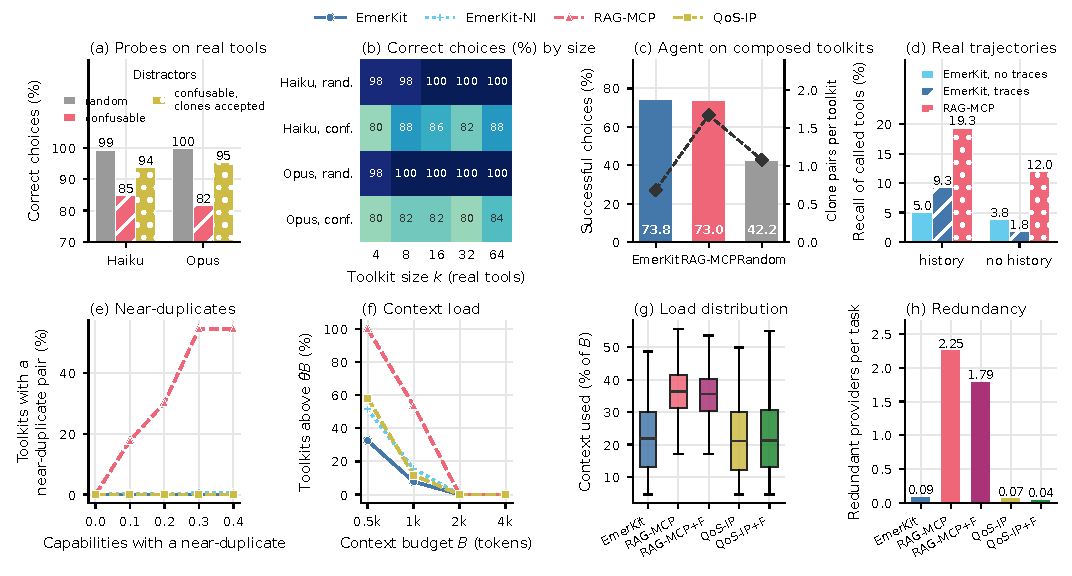
\includegraphics[width=\textwidth]{fig_rq1.pdf}
\caption{Quality of toolkits. (a,\,b) Selection probes on real tool definitions. (c) Agent success and clone pairs on composed toolkits. (d) Recall of the tools called in real trajectories. (e--h) Near-duplicates, context load, load distribution, and redundancy of the toolkits.}\label{fig:rq1}
\end{figure}

\paragraph{Tool selection by agents on real definitions.} The first experiment tests whether co-present tools degrade the choice of an agent, which is the premise of the quality model, and it estimates the interaction terms. A model that is not probed wrote, for each of 500 real tools of the Toucan catalogue, a request that this tool should serve. The probed model then chose among the target and $k-1$ other real tools, with $k$ between 4 and 64; the other tools are either drawn at random or are the tools of other servers whose descriptions are closest to the target. Fig.~\ref{fig:rq1}a shows that both models choose the target in more than 99\% of the probes with random distractors, but only in \RAfiveHaikuConf\% (Haiku) and \RAfiveOpusConf\% (Opus) of the probes with confusable distractors. Fig.~\ref{fig:rq1}b shows that the size of the toolkit has no visible effect. A logistic model fitted on half of the probes confirms both observations: confusable distractors lower the log-odds of a correct choice by \RAfiveCoefConf{} ($p\RAfivePConf$), whereas the coefficient of the log of the load is \RAfiveCoefLoad{} ($p=\RAfivePLoad$). The interference index of the paper, fitted on the same half, predicts the errors of the other half with an AUC of \RFitAuc, against \RFitAucBase{} without it, and the fitted saturation weight is \RFitLamC. A closer inspection reveals that \RClShare\% of the errors select a clone of the target, that is, the same tool published by another server; when clones are accepted, accuracy under confusable distractors reaches \RClHaiku\% and \RClOpus\%. These results support the interference component of the quality model and show that it is predictive. They do not support the saturation component for these models and for loads of up to 64 real definitions; we therefore set its weight to zero and keep the term for smaller agents, for which it remains to be tested. The prevalence of clones also indicates that interference is a governance issue, because a clone serves the request but may belong to a server with another receiver role.

A second experiment examines whether composing against interference helps an agent. For the same 500 requests, the 16 most relevant tools form a common pool from which 8 tools are kept by three strategies: the 8 most relevant tools (RAG-MCP), the subset that maximizes relevance minus the fitted interference, found by enumeration (\sysname{}), and a random subset. A choice is counted as successful when the agent selects the target or one of its clones. As Fig.~\ref{fig:rq1}c shows, \sysname{} succeeds in \RSixEmk\% of the requests and RAG-MCP in \RSixRag\%, a difference that is not significant ($p=\RSixP$), whereas the random toolkit succeeds in \RSixRnd\%. \sysname{} nevertheless keeps \RSixEmkClones{} clone pairs per toolkit against \RSixRagClones{} for RAG-MCP. Removing clones therefore does not change the success of this agent, which picks the target or a clone in about 95\% of the cases when one is present; its benefit lies in controlling which provider receives the data.

\paragraph{Structure of the composed toolkits.} We next measure what the quality model changes in the toolkits themselves on the synthetic catalogue. When up to 40\% of the capabilities have a near-duplicate provider, RAG-MCP returns a near-duplicate pair in up to \RARagCpMax\% of its toolkits, whereas \sysname{} returns none (Fig.~\ref{fig:rq1}e). Under a budget of 1{,}000 tokens, \RAOverEmk\% of the toolkits of \sysname{} exceed the threshold $\theta B$, against \RAOverNoInt\% for \sysname{}-NI, \RAOverZeng\% for QoS-IP, and \RAOverRag\% for RAG-MCP, which exceeds the budget itself in \RARagExceed\% of the tasks at 500 tokens (Fig.~\ref{fig:rq1}f). The distribution of the load in Fig.~\ref{fig:rq1}g and the redundancy in Fig.~\ref{fig:rq1}h lead to the same conclusion: methods that count each capability once, namely \sysname{} and QoS-IP, use about a fifth of the budget and almost no redundant provider, whereas relevance retrieval accumulates overlapping tools, with \RARagMcpRed{} redundant providers per task.

\paragraph{Evidence from real trajectories.} The last experiment of this group assesses trace evidence and co-usage on real requests. Toolkits are compared with the tools that Toucan trajectories actually called; the capabilities of a real tool are the categories of its server, and those of a request are its two closest categories. Fig.~\ref{fig:rq1}d shows that, when tools have a usage history, trace evidence raises the recall of \sysname{} from \RSvWarmNoTraces\% to \RSvWarmTraces\%, and that it lowers it from \RSvColdNoTraces\% to \RSvColdTraces\% for tools without history, while RAG-MCP reaches \RSvWarmRag\% and \RSvColdRag\%. Co-usage has no measurable effect, since at most one tool per category is selected. Trace evidence thus helps but carries a cold-start bias. More importantly, composition by capabilities requires a vocabulary as fine as the needs it serves: with categories as coarse as those of servers, relevance retrieval finds real tools better than \sysname{}.

\section{Norm Compliance and Risk Guarantee (RQ2)}\label{sec:res-h2}

\begin{table}[!ht]\centering
\caption{Reference comparison over \RNTasks{} tasks and \RNSeeds{} seeds (rates in \%). Best deployable value in bold.}\label{tab:main}
\scriptsize\setlength{\tabcolsep}{4pt}\begin{tabular}{lrrrrrrrrrrrrr}\toprule
& \multicolumn{7}{c}{All tasks} & \multicolumn{6}{c}{Valid toolkits by pedagogical type $\uparrow$} \\ \cmidrule(lr){2-8}\cmidrule(lr){9-14}
Method & Equip. $\uparrow$ & Valid $\uparrow$ & DFR $\downarrow$ & QoS $\downarrow$ & Red. $\downarrow$ & Load $\downarrow$ & Size & Acq. & Prac. & Form. & Summ. & Disc. & Prod. \\ \midrule
\sysname{} & 69.8 & 67.3 & \textbf{3.3} & 0.2 & 0.09 & 22.3 & 2.52 & \textbf{83.2} & 56.8 & 58.0 & 53.6 & 78.8 & 73.6 \\
\sysname{} ($\xi{=}0.10$) & 76.1 & 71.1 & 6.5 & 0.2 & 0.08 & 22.7 & 2.58 & 81.6 & 60.4 & 60.0 & 56.8 & \textbf{84.8} & 82.8 \\
RAG-MCP & \textbf{100.0} & 8.1 & 78.9 & 55.6 & 2.25 & 36.8 & 4.00 & 27.6 & 0.0 & 0.8 & 0.0 & 17.6 & 2.4 \\
RAG-MCP+F & \textbf{100.0} & 31.3 & 20.5 & 30.1 & 1.79 & 35.6 & 4.00 & 27.6 & 24.0 & 43.2 & 39.6 & 31.2 & 22.4 \\
QoS-IP & 99.5 & 54.5 & 45.2 & 0.6 & 0.07 & \textbf{22.1} & 2.55 & 76.4 & 33.2 & 38.0 & 28.0 & 78.4 & 73.2 \\
QoS-IP+F & 82.0 & \textbf{72.6} & 11.5 & \textbf{0.1} & \textbf{0.04} & 22.4 & 2.55 & 78.4 & \textbf{64.4} & \textbf{60.8} & \textbf{59.2} & 78.0 & \textbf{94.8} \\
\midrule
Oracle & 78.9 & 78.7 & 0.0 & 0.2 & 0.07 & 22.4 & 2.52 & 89.2 & 70.8 & 62.0 & 58.0 & 96.0 & 96.4 \\
\bottomrule\end{tabular}

\end{table}

\begin{figure}[!ht]\centering
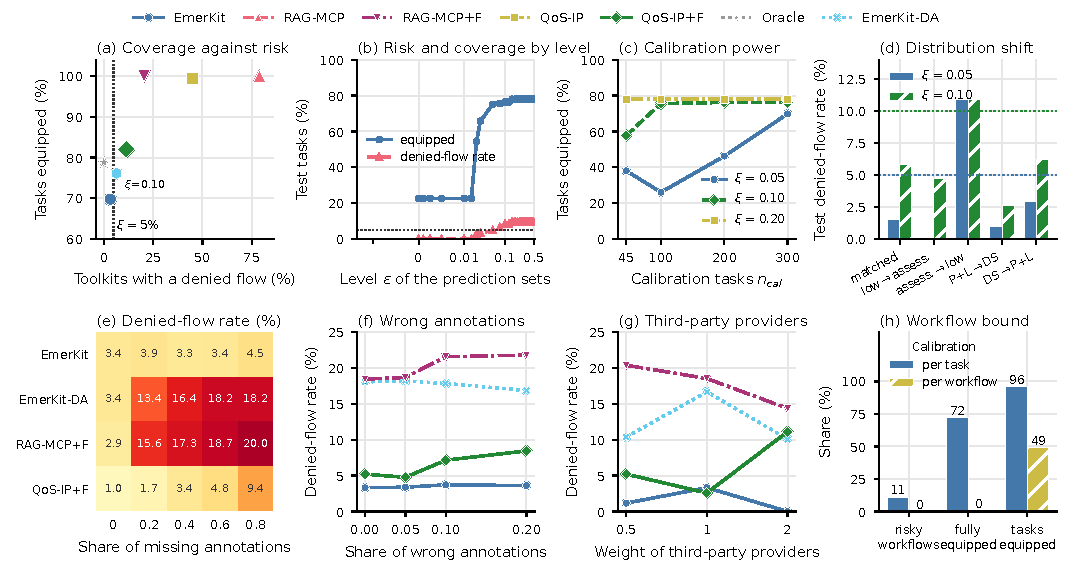
\includegraphics[width=\textwidth]{fig_rq2.pdf}
\caption{Norm compliance and risk guarantee. (a) Coverage against risk. (b) Risk and coverage by level $\epsilon$. (c) Effect of the calibration set. (d) Calibration under distribution shift. (e--g) Denied-flow rate under missing annotations, wrong annotations, and third-party providers. (h) Task-level and workflow-level calibration.}\label{fig:rq2}
\end{figure}

\paragraph{Comparison with the baselines.} The reference comparison measures coverage, validity, and risk for all methods on the same tasks. Table~\ref{tab:main} and Fig.~\ref{fig:rq2}a show that \sysname{} returns toolkits with a denied flow in \RAEmerkitDfr\% of the equipped tasks, whereas RAG-MCP reaches \RARagMcpDfr\%, QoS-IP \RAZengDfr\%, and their filtered variants \RARagMcpPlusFilterDfr\% and \RAZengPlusFilterDfr\%. \sysname{} equips \RAEmerkitEq\% of the tasks, against \RAOracleEq\% for the Oracle. Its share of valid toolkits, \RAEmerkitValid\%, exceeds that of RAG-MCP, RAG-MCP+F, and QoS-IP, but not that of QoS-IP+F, which reaches \RAZengPlusFilterValid\%. When \sysname{} is calibrated at $\xi=0.10$, it equips \RAEmerkitXiEq\% of the tasks with \RAEmerkitXiDfr\% of denied flows. The breakdown by pedagogical type in Table~\ref{tab:main} shows that validity is lowest for practice and assessment tasks with every method, and that the gap between \sysname{} and the Oracle is largest for production and discussion tasks. These results confirm that relevance and QoS are blind to data flows and that a filter on declared annotations cannot see what is not declared. They also show that safety has a cost in coverage: the gap to the Oracle is the price of uncertain labels, and QoS-IP+F obtains its additional valid toolkits with a denied-flow rate more than three times higher.

\paragraph{Calibration, sample size, and distribution shift.} We then check the bound of Proposition 3 and its cost. Over the twelve combinations of the target risk $\xi$ and the number of calibration tasks $n_{cal}$, the test denied-flow rate stays below $\xi$ and reaches at most \RBMaxDfrRatio{} times the target. Fig.~\ref{fig:rq2}b illustrates the trade-off controlled by the level $\epsilon$, and Fig.~\ref{fig:rq2}c shows the role of statistical power: at $\xi=0.05$, the share of equipped tasks grows from \RBEqHundred\% with 100 calibration tasks to \RBEqThree\% with 300, whereas the purely worst-case check ($\epsilon=0$) equips only \RBEqEpsZero\% of the tasks. Table~\ref{tab:shift} and Fig.~\ref{fig:rq2}d examine what happens when the calibration tasks do not follow the distribution of the test tasks. The bound holds when calibration and test are matched (\RXsixMatchDfr\% of denied flows at $\xi=0.05$) and under a change of domain (at most \RXsixDomMax\%). It becomes very conservative when the level is calibrated on low-stakes types and applied to assessment types (\RXsixLowEq\% of tasks equipped), and it is violated in the opposite direction, with \RXsixAssessDfr\% of denied flows. The guarantee is therefore valid for the calibrated task distribution only, and calibration must cover the pedagogical types that are deployed, as the sample-size rule of the paper already requires for statistical power.

\begin{table}[!ht]\centering
\caption{Calibration under distribution shift: calibrated level, test denied-flow rate (\%), and equipped tasks (\%). Underlined rates exceed the target.}\label{tab:shift}
\scriptsize\setlength{\tabcolsep}{6pt}\begin{tabular}{lrrrrrr}\toprule
& \multicolumn{3}{c}{$\xi=0.05$} & \multicolumn{3}{c}{$\xi=0.10$} \\ \cmidrule(lr){2-4}\cmidrule(lr){5-7}
Calibration $\to$ test & $\hat\epsilon$ & DFR & Equip. & $\hat\epsilon$ & DFR & Equip. \\ \midrule
Matched (all types, all domains) & 0.072 & 1.5 & 67.3 & 0.350 & 5.8 & 87.4 \\
Low-stakes types $\to$ assessment types & 0.017 & 0.0 & 21.0 & 0.233 & 4.7 & 81.1 \\
Assessment types $\to$ low-stakes types & 0.350 & \underline{10.9} & 91.4 & 0.350 & \underline{10.9} & 91.4 \\
Programming, language $\to$ data science & 0.053 & 1.0 & 52.4 & 0.225 & 2.6 & 89.2 \\
Data science $\to$ programming, language & 0.083 & 2.9 & 84.7 & 0.350 & 6.2 & 86.6 \\
\bottomrule\end{tabular}

\end{table}

\begin{table}[!ht]\centering
\caption{Denied-flow rate (\%) under imperfect metadata and under different norm bases. Best value in bold.}\label{tab:robust}
\scriptsize\setlength{\tabcolsep}{4pt}\begin{tabular}{lrrrrrrrrrrrrrr}\toprule
& \multicolumn{5}{c}{Missing annotations} & \multicolumn{3}{c}{Wrong annotations} & \multicolumn{3}{c}{Third-party weight} & \multicolumn{3}{c}{Norm profile} \\ \cmidrule(lr){2-6}\cmidrule(lr){7-9}\cmidrule(lr){10-12}\cmidrule(lr){13-15}
Method & 0 & 0.2 & 0.4 & 0.6 & 0.8 & 0 & 0.1 & 0.2 & 0.5 & 1 & 2 & perm. & std & strict \\ \midrule
\sysname{} & 3.4 & 3.9 & \textbf{3.3} & \textbf{3.4} & \textbf{4.5} & \textbf{3.3} & \textbf{3.7} & \textbf{3.6} & \textbf{1.2} & 3.3 & \textbf{0.0} & \textbf{1.3} & \textbf{1.6} & \textbf{0.7} \\
\sysname{}-DA & 3.4 & 13.4 & 16.4 & 18.2 & 18.2 & 18.1 & 17.8 & 16.8 & 10.4 & 16.7 & 10.1 & 10.6 & 12.5 & 14.6 \\
RAG-MCP+F & 2.9 & 15.6 & 17.3 & 18.7 & 20.0 & 18.4 & 21.6 & 21.8 & 20.4 & 18.5 & 14.4 & 15.4 & 17.7 & 21.5 \\
QoS-IP+F & \textbf{1.0} & \textbf{1.7} & 3.4 & 4.8 & 9.4 & 5.2 & 7.1 & 8.4 & 5.2 & \textbf{2.6} & 11.1 & 6.7 & 6.1 & 7.2 \\
\bottomrule\end{tabular}

\end{table}

\paragraph{Robustness to imperfect metadata and to norms.} This experiment tests how each method reacts to what providers publish and to the norm base. Table~\ref{tab:robust} and Fig.~\ref{fig:rq2}e--g show that, when missing annotations vary from 0 to 80\% and wrong ones from 0 to 20\%, the denied-flow rate of \sysname{} stays between \RBtwoEmkMin\% and \RBtwoEmkMax\%. In contrast, \sysname{}-DA, which trusts declared annotations, goes from \RBtwoDeclMzero\% to \RBtwoDeclMeight\%, and the filtered baselines reach \RBtwoRagMax\% (RAG-MCP+F) and \RBtwoZengMax\% (QoS-IP+F). Under three norm profiles and three shares of third-party providers, the rate of \sysname{} never exceeds \RBthreeEmkMax\%, whereas QoS-IP+F reaches \RBthreeZengHigh\% when third parties dominate. The risk of \sysname{} thus does not depend on how much providers declare. Wrong annotations make it more cautious, since it equips \RBtwoEqWzero\% and then \RBtwoEqWtwenty\% of the tasks, but they do not make it riskier.

\paragraph{Live enactment through the gateway.} To confront the flow graph with real executions, every toolkit was enacted on executable servers. Over \RFoneN{} toolkits, the gateway exposed only the tools of the toolkit and refused every other call, and a policy that calls every tool with everything its parameters can carry realised exactly the predicted flows in \RFoneExact\% of the toolkits. A Claude agent that enacted \RFlN{} tasks realised \RFlRealised\% of the possible flows and none outside the predicted set. On these servers, the flow graph is therefore exact, and an agent realises a subset of what a toolkit makes possible, which is what the worst-case reading assumes.

\paragraph{From task-level to workflow-level guarantees.} The bound of Proposition 3 is stated per task, and Fig.~\ref{fig:rq2}h quantifies its consequence for whole workflows. With the task-level calibration, \RWcTaskRisk\% of the workflows contain a risky toolkit and \RWcTaskAll\% are fully equipped. With the workflow-level calibration, the share of risky workflows falls to \RWcWfRisk\%, but only \RWcWfAll\% of the workflows remain fully equipped. A bound per task does not bound the risk of a workflow, and a bound per workflow is attainable only at a high price in coverage.

\section{Composition and Revision (RQ3)}\label{sec:res-h3}

\begin{figure}[!ht]\centering
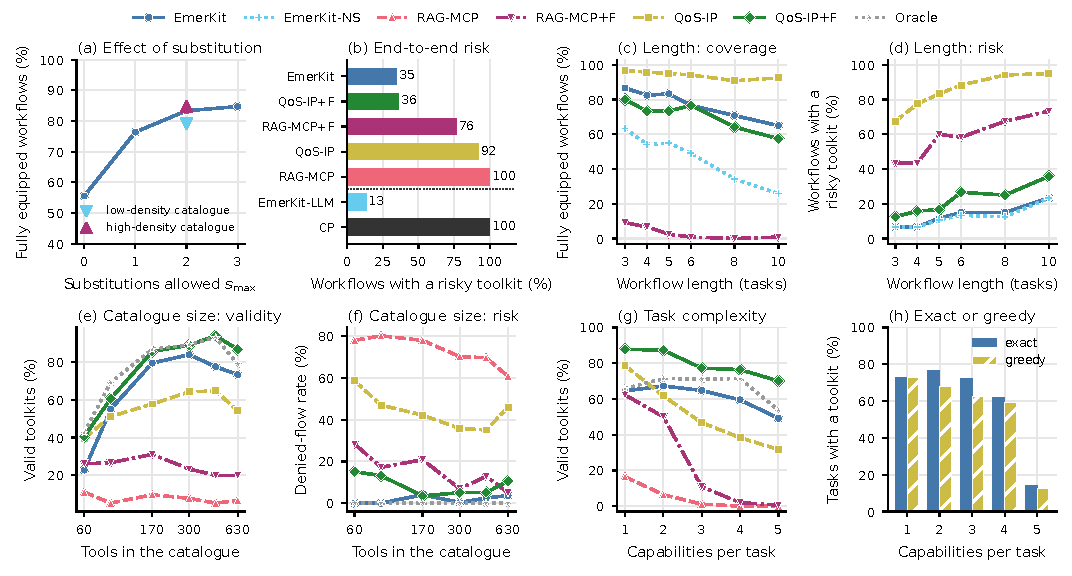
\includegraphics[width=\textwidth]{fig_rq3.pdf}
\caption{Composition and revision. (a) Substitution. (b) Workflows with a risky toolkit, end to end. (c,\,d) Coverage and risk against workflow length. (e,\,f) Validity and risk against catalogue size. (g) Validity against the number of capabilities per task. (h) Exact and greedy composition.}\label{fig:rq3}
\end{figure}

\begin{table}[!ht]\centering
\caption{End-to-end comparison (rates in \%): tasks equipped, fully equipped workflows, workflows with a risky toolkit, and objectives covered. Top: rule-based generator; bottom: language model. Best value in bold.}\label{tab:e2e}
\scriptsize\setlength{\tabcolsep}{3pt}\begin{tabular}{lrrrr}\toprule
Method & Tasks eq. $\uparrow$ & Fully eq. $\uparrow$ & Risky $\downarrow$ & Obj. $\uparrow$ \\ \midrule
\sysname{}-NS & 92.3 & 55.6 & 34.7 & 99.3 \\
\sysname{} & 97.8 & 83.3 & 34.7 & \textbf{100.0} \\
RAG-MCP & 28.4 & 0.0 & 100.0 & \textbf{100.0} \\
RAG-MCP+F & 46.1 & 0.0 & 76.4 & \textbf{100.0} \\
QoS-IP & 98.8 & \textbf{93.1} & 91.7 & \textbf{100.0} \\
QoS-IP+F & 90.2 & 56.9 & 36.1 & \textbf{100.0} \\
\midrule
\sysname{}-LLM & 84.8 & -- & \textbf{13.3} & \textbf{100.0} \\
CP & \textbf{100.0} & -- & 100.0 & 70.8 \\
\bottomrule\end{tabular}

\end{table}

\paragraph{End-to-end composition and substitution.} This experiment evaluates substitution and compares complete pipelines, from the request to the composed workflow. Table~\ref{tab:e2e} and Fig.~\ref{fig:rq3}a show that, behind the rule-based generator, substitution raises the share of fully equipped workflows from \RCtwoAllZero\% (\sysname{}-NS) to \RCtwoAllTwo\% with at most two substitutions. In this setting, \RCtwoSub\% of the tasks are substituted, with \RCtwoPrereq{} prerequisite violation and \RCtwoPres{} substitution outside the preservation relation, whereas QoS-IP+F equips every task of only \RCtwoZfAll\% of the workflows. With a language model, CP equips every task, but all of its compositions contain a toolkit with a denied flow and it covers \RCoCpObj\% of the target concepts (Fig.~\ref{fig:rq3}b). \sysname{}-LLM obtains a valid workflow for \RCoLgValid\% of the requests, covers all targets, and \RCoLgRisk\% of its workflows contain a risky toolkit. Substitution thus turns incomplete workflows into complete ones without leaving the catalogue approved by instructors, and a language model alone composes plausible but non-compliant toolkits.

\begin{table}[!ht]\centering
\caption{Effect of the number of capabilities required per task (rates in \%). Best deployable value in bold.}\label{tab:caps}
\scriptsize\setlength{\tabcolsep}{5pt}\begin{tabular}{lrrrrrrrrrr}\toprule
& \multicolumn{5}{c}{Valid toolkits (\%) $\uparrow$} & \multicolumn{5}{c}{DFR (\%) $\downarrow$} \\ \cmidrule(lr){2-6}\cmidrule(lr){7-11}
Method & 1 & 2 & 3 & 4 & 5 & 1 & 2 & 3 & 4 & 5 \\ \midrule
\sysname{} & 64.4 & 67.2 & 64.7 & 59.4 & 49.2 & \textbf{0.0} & \textbf{0.8} & \textbf{5.2} & \textbf{10.4} & \textbf{7.3} \\
RAG-MCP & 16.4 & 6.4 & 1.1 & 0.0 & 0.0 & 76.9 & 81.7 & 80.8 & 82.5 & 83.1 \\
RAG-MCP+F & 62.2 & 50.0 & 10.8 & 1.9 & 0.6 & 17.8 & 20.0 & 21.1 & 21.9 & 24.4 \\
QoS-IP & 78.6 & 61.7 & 46.7 & 38.3 & 31.7 & 16.0 & 38.3 & 53.3 & 61.7 & 68.3 \\
QoS-IP+F & \textbf{87.8} & \textbf{87.2} & \textbf{77.2} & \textbf{76.4} & \textbf{70.0} & \textbf{0.0} & 3.7 & 11.1 & 13.2 & 18.1 \\
\midrule
Oracle & 65.8 & 71.4 & 71.1 & 71.4 & 53.6 & 0.0 & 0.0 & 0.0 & 0.0 & 0.0 \\
\bottomrule\end{tabular}

\end{table}

\begin{table}[!ht]\centering
\caption{Effect of the workflow length, in tasks (rates in \%). Best value in bold.}\label{tab:len}
\scriptsize\setlength{\tabcolsep}{5pt}\begin{tabular}{lrrrrrrrrrrrr}\toprule
& \multicolumn{6}{c}{Fully equipped workflows (\%) $\uparrow$} & \multicolumn{6}{c}{Workflows with a risky toolkit (\%) $\downarrow$} \\ \cmidrule(lr){2-7}\cmidrule(lr){8-13}
Method & 3 & 4 & 5 & 6 & 8 & 10 & 3 & 4 & 5 & 6 & 8 & 10 \\ \midrule
\sysname{} & 86.7 & 82.5 & 83.3 & 76.7 & 70.8 & 65.0 & \textbf{6.7} & \textbf{6.7} & 11.7 & 15.0 & 15.0 & \textbf{23.3} \\
\sysname{}-NS & 63.3 & 54.2 & 55.0 & 49.2 & 34.2 & 25.8 & \textbf{6.7} & \textbf{6.7} & \textbf{10.8} & \textbf{13.3} & \textbf{12.5} & \textbf{23.3} \\
RAG-MCP & 3.3 & 0.8 & 0.0 & 0.0 & 0.0 & 0.0 & 96.7 & 99.2 & 100.0 & 100.0 & 100.0 & 100.0 \\
RAG-MCP+F & 9.2 & 6.7 & 2.5 & 0.8 & 0.0 & 0.8 & 43.3 & 43.3 & 60.0 & 58.3 & 67.5 & 73.3 \\
QoS-IP & \textbf{96.7} & \textbf{95.8} & \textbf{95.0} & \textbf{94.2} & \textbf{90.8} & \textbf{92.5} & 67.5 & 77.5 & 83.3 & 88.3 & 94.2 & 95.0 \\
QoS-IP+F & 80.0 & 73.3 & 73.3 & 76.7 & 64.2 & 57.5 & 12.5 & 15.8 & 16.7 & 26.7 & 25.0 & 35.8 \\
\bottomrule\end{tabular}

\end{table}

\paragraph{Complexity of requests.} We study how the methods behave when requests become more demanding, first in the number of capabilities required per task and then in the length of the workflow. Table~\ref{tab:caps} and Fig.~\ref{fig:rq3}g show that validity decreases for every method as tasks require more capabilities. \sysname{} goes from \RXtwoEmkOne\% of valid toolkits with one capability to \RXtwoEmkFive\% with five, close to the Oracle (\RXtwoOraFive\%), while RAG-MCP+F collapses to \RXtwoRagFive\%. QoS-IP+F keeps the highest validity (\RXtwoZfFive\% with five capabilities), but its denied-flow rate grows to \RXtwoZfDfrFive\%; that of \sysname{} peaks at \RXtwoEmkDfrMax\%, above the target, because tasks with many capabilities differ from the tasks used at the fixed level. Table~\ref{tab:len} and Fig.~\ref{fig:rq3}c,\,d report the effect of the workflow length. The share of fully equipped workflows of \sysname{} decreases from \RXfourEmkThree\% for three tasks to \RXfourEmkTen\% for ten, against \RXfourNsTen\% without substitution and \RXfourZfTen\% for QoS-IP+F. QoS-IP equips \RXfourZTen\% of the ten-task workflows, but \RXfourZRiskTen\% of them contain a risky toolkit. The risk of \sysname{} accumulates with length, from \RXfourEmkRiskThree\% to \RXfourEmkRiskTen\% of risky workflows, and remains below that of QoS-IP+F (\RXfourZfRiskTen\%). Longer and more demanding requests therefore widen the difference between methods: substitution preserves coverage, and the per-task guarantee limits, without eliminating, the accumulation of risk.

\begin{table}[!ht]\centering
\caption{Exact and greedy composition by shortlist bound $N$ and capabilities per task $|R|$.}\label{tab:greedy}
\scriptsize\setlength{\tabcolsep}{3pt}\begin{tabular}{rrrrrrrr}\toprule
& & \multicolumn{2}{c}{Tasks equipped (\%)} & \multicolumn{2}{c}{Greedy objective} & \multicolumn{2}{c}{Median time (ms)} \\ \cmidrule(lr){3-4}\cmidrule(lr){5-6}\cmidrule(lr){7-8}
$N$ & $|R|$ & exact & greedy & ratio & optimal (\%) & exact & greedy \\ \midrule
10 & 3 & \textbf{48.5} & 40.0 & 0.999 & 99.1 & 4.6 & \textbf{0.7} \\
20 & 1 & \textbf{73.0} & 73.0 & 1.000 & 100.0 & 14.4 & \textbf{0.5} \\
20 & 2 & \textbf{76.7} & 67.8 & 0.996 & 94.0 & 20.6 & \textbf{0.9} \\
20 & 3 & \textbf{72.2} & 62.6 & 0.995 & 92.3 & 135.8 & \textbf{1.1} \\
20 & 4 & \textbf{61.9} & 59.3 & 0.996 & 83.0 & 126.8 & \textbf{1.2} \\
20 & 5 & \textbf{14.1} & 12.2 & 0.999 & 63.6 & 10.4 & \textbf{1.1} \\
50 & 3 & \textbf{90.0} & 77.4 & 0.993 & 89.4 & 189.6 & \textbf{1.6} \\
100 & 3 & \textbf{90.0} & 77.4 & 0.993 & 89.4 & 185.0 & \textbf{1.6} \\
\bottomrule\end{tabular}

\end{table}

\paragraph{Exact versus greedy composition.} Since Proposition 1 gives a greedy guarantee under a condition, we compare the exact composer with a greedy composer that uses the same shortlist, coefficients, and constraints and serves capabilities one at a time. Table~\ref{tab:greedy} and Fig.~\ref{fig:rq3}h show that, when both composers return a toolkit, the greedy objective is on average \RXfiveRatio{} times the optimum. The difference lies in feasibility: the greedy composer fails on up to \RXfiveLoss\% of the tasks that the exact composer equips, for example \RXfiveGrFifty\% against \RXfiveExFifty\% of tasks equipped with a shortlist of 50 candidates. The exact composer needs at most \RXfiveExMs{}~ms per task in median, against \RXfiveGrMs{}~ms for the greedy one. Exact composition is thus valuable because of the hard constraints on flows, budget, and QoS, which a myopic choice often cannot satisfy, rather than because of the objective.

\section{Scalability}\label{sec:res-scal}

\begin{table}[!ht]\centering
\caption{Effect of the catalogue size, in tools (rates in \%; last column: median composition time per task at the largest size). Best deployable value in bold.}\label{tab:scale}
\scriptsize\setlength{\tabcolsep}{4pt}\begin{tabular}{lrrrrrrrrrrrrr}\toprule
& \multicolumn{6}{c}{Valid toolkits (\%) $\uparrow$ by catalogue size} & \multicolumn{6}{c}{DFR (\%) $\downarrow$ by catalogue size} & ms \\ \cmidrule(lr){2-7}\cmidrule(lr){8-13}\cmidrule(lr){14-14}
Method & 60 & 90 & 170 & 300 & 450 & 630 & 60 & 90 & 170 & 300 & 450 & 630 & 630 \\ \midrule
\sysname{} & 22.8 & 55.0 & 79.4 & 83.9 & 77.5 & 73.3 & \textbf{0.0} & \textbf{0.0} & 4.0 & \textbf{0.3} & \textbf{2.4} & \textbf{3.6} & 24.9 \\
RAG-MCP & 11.1 & 5.3 & 9.7 & 7.8 & 5.3 & 6.7 & 78.1 & 80.3 & 78.1 & 70.3 & 69.7 & 60.8 & 1.5 \\
RAG-MCP+F & 26.1 & 26.7 & 31.1 & 23.3 & 20.0 & 20.0 & 28.3 & 17.2 & 20.8 & 6.9 & 12.8 & 5.0 & \textbf{0.9} \\
QoS-IP & 39.7 & 51.1 & 57.8 & 64.2 & 64.7 & 54.2 & 58.7 & 47.0 & 42.2 & 35.8 & 35.1 & 45.8 & 4.3 \\
QoS-IP+F & \textbf{40.6} & \textbf{60.6} & \textbf{85.6} & \textbf{88.9} & \textbf{93.9} & \textbf{86.7} & 15.1 & 13.1 & \textbf{3.4} & 5.0 & 5.1 & 10.6 & 4.5 \\
\midrule
Oracle & 42.8 & 69.2 & 86.7 & 89.2 & 93.1 & 78.9 & 0.0 & 0.0 & 0.0 & 0.0 & 0.0 & 0.0 & 28.8 \\
\bottomrule\end{tabular}

\end{table}

\begin{figure}[!ht]\centering
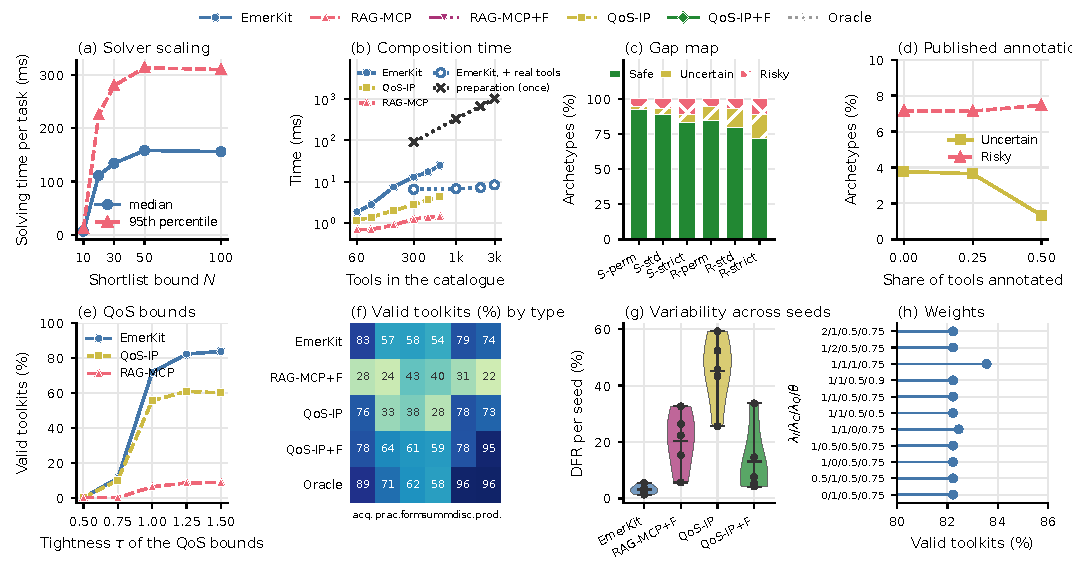
\includegraphics[width=\textwidth]{fig_rq4.pdf}
\caption{Scalability, gap map, and sensitivity. (a) Solver time against the shortlist bound. (b) Composition time against catalogue size. (c) Gap map by catalogue (S: synthetic, R: with MCP-tools) and norm profile. (d) Effect of published annotations. (e) QoS bounds. (f) Valid toolkits by pedagogical type. (g) Denied-flow rate across seeds. (h) Weights of the quality model.}\label{fig:rq4}
\end{figure}

\paragraph{Catalogue size.} This experiment varies the number of providers per capability, so that the synthetic catalogue grows from \RXoneMin{} to \RXoneMax{} tools with its ground truth. Table~\ref{tab:scale} and Fig.~\ref{fig:rq3}e,\,f show that the validity of \sysname{} rises from \RXoneEmkValidMin\% with the smallest catalogue, in which most tasks have no admissible provider, to \RXoneEmkValidMax\%, and that its denied-flow rate never exceeds \RXoneEmkDfrMax\%. QoS-IP+F reaches up to \RXoneZfValidMax\% of valid toolkits but its denied-flow rate reaches \RXoneZfDfrMax\%, and RAG-MCP stays below 12\% of valid toolkits at every size. A larger catalogue thus helps the methods that reason on capabilities and constraints, because it offers more admissible alternatives, and it does not help relevance retrieval.

\paragraph{Solver and catalogue scaling.} With up to 100 candidates per task, the median solving time stays below \RCthreeMedMax{}~s and the 95th percentile below \RCthreePmax{}~s, without any time-out (Fig.~\ref{fig:rq4}a). The median composition time of \sysname{} grows from about 2~ms to \RXoneEmkMs{}~ms between the smallest and the largest synthetic catalogue, against \RXoneZMs{}~ms for QoS-IP (Fig.~\ref{fig:rq4}b). When up to 2{,}960 real tools from MCP-tools and Toucan are added, preparation takes \RCfourPrep{}~s, a task is composed in \RCfourEmkSmall{} to \RCfourEmkLarge{}~ms, and memory stays below \RCfourMem{}~MB. Exact composition is therefore practical at these sizes, and the main cost lies in the preparation, which is performed once per catalogue snapshot.

\section{Gap Map of the Ecosystem (RQ4)}\label{sec:res-h4}

The gap map is expected to expose actionable levers. On the synthetic catalogue with the standard norms, \REoneSafeSyn\% of the demand-weighted archetypes are safe, \REoneUncSyn\% are uncertain, and \REoneRiskStd\% are risky. Strict norms raise the risky share to \REoneRiskStrict\%, and adding the unannotated MCP-tools raises the uncertain share to \REoneUncMix\% (Fig.~\ref{fig:rq4}c). When providers publish correct annotations for half of the tools, the uncertain share falls to \REtwoUncHalf\% (Fig.~\ref{fig:rq4}d). The classes thus react to the levers they are meant to expose: norms create risky archetypes, and undocumented tools create uncertain ones. The map tells providers which annotations to publish and institutions which tools to commission.

\section{Ablation and Sensitivity Analysis}\label{sec:res-sens}

\begin{table}[!ht]\centering
\caption{Ablation of the components of \sysname{}: equipped, valid, denied-flow rate, QoS violations, and load (\%), and redundancy. Best value in bold.}\label{tab:abl}
\scriptsize\setlength{\tabcolsep}{3pt}\begin{tabular}{lrrrrrr}\toprule
Variant & Eq. $\uparrow$ & Valid $\uparrow$ & DFR $\downarrow$ & QoS $\downarrow$ & Red. $\downarrow$ & Load $\downarrow$ \\ \midrule
\sysname{} (full) & 69.8 & \textbf{67.3} & \textbf{3.3} & 0.2 & 0.09 & \textbf{22.3} \\
additive utility & 69.8 & 66.7 & 4.5 & \textbf{0.0} & 1.10 & 30.4 \\
declared annotations (DA) & \textbf{80.9} & 65.4 & 19.0 & 0.2 & \textbf{0.08} & 23.1 \\
no QoS & 76.5 & 39.9 & 4.1 & 46.1 & 0.23 & 24.7 \\
no interactions (NI) & 69.8 & \textbf{67.3} & \textbf{3.3} & 0.2 & 0.14 & 22.7 \\
\bottomrule\end{tabular}

\end{table}

Table~\ref{tab:abl} removes one component of \sysname{} at a time. Replacing the prediction sets by declared annotations equips more tasks but multiplies the denied-flow rate by almost six. The additive utility multiplies redundancy by twelve, and removing QoS leads \RDNoQosQviol\% of the toolkits to violate their bounds. Without the interaction terms, coverage and risk are unchanged and redundancy rises from \RDFullEmerkitRed{} to \RDNoInteractionsRed.

The results are stable with respect to the parameters. The share of valid toolkits stays between \RDtwoValidMin\% and \RDtwoValidMax\% over eleven settings of $\lambda_I$, $\lambda_C$, $\lambda_Q$, and $\theta$ (Fig.~\ref{fig:rq4}h). The tightness of the QoS bounds matters more: with $\tau=1.25$, \sysname{} returns \RAfourEmk\% of valid toolkits at the fixed level, against \RAfourZeng\% for QoS-IP, and both fall near 10\% at $\tau=0.75$ (Fig.~\ref{fig:rq4}e). Fig.~\ref{fig:rq4}f details validity by pedagogical type, and Fig.~\ref{fig:rq4}g shows that the denied-flow rate of \sysname{} varies little across seeds, whereas that of the baselines varies widely. The pedagogical parameters were also submitted to three language models, which judged every norm cell, substitution pair, and fit value. Their majority agrees with the norm base on \RJnAgree\% of the cells ($\kappa=\RJnKappa$) and with the substitution catalogue on \RJsAgree\% of the pairs ($\kappa=\RJsKappa$); with their norms and catalogue, \sysname{} keeps a denied-flow rate of \RPonePanelDfr\%, against \RPoneStandardDfr\% with ours, and \RPtwoPanelAll\% of fully equipped workflows, against \RPtwoStandardAll\%. Finally, the labels of 210 real tools come from a static analysis of their code followed by a model review, and Sonnet agrees with an independent review of 40 tools on \RAuSonnetAgree{} of them.

\section{Threats to Validity}\label{sec:threats}

Regarding internal validity, the measures of norm compliance need a ground truth and therefore use synthetic servers, whose descriptions are cleaner than real ones; real catalogues are used in the selection probes, the agent experiment, the trajectories, the scalability experiment, and the gap map. Regarding construct validity, the pedagogical parameters and the audit labels of real tools come from model judgements and not from instructors or human auditors, and the models of the panel share a family, which may inflate their agreement. Regarding external validity, all language models come from one provider: interference is supported for these models, saturation is not, and smaller open models remain to be tested. The guarantee is stated per task and for the calibrated task distribution, as the shift experiment shows, and it must be recalibrated with each registry snapshot. The end-to-end experiments that involve a language model use three seeds and a few dozen requests or tasks each.


\part*{Part II: Detailed tables by series}
\section{Preparation quality }
Capability extraction reaches a precision of \RCapPrec\% and a recall of \RCapRec\%; synthetic descriptions are easier than real ones, so this figure is optimistic. Label classifiers reach an accuracy between \RLabAccMin\% and \RLabAccMax\% depending on the label. The empirical coverage of the conformal sets is \RConfCovFive\%, \RConfCovTen\%, and \RConfCovTwenty\% for $\epsilon=0.05$, $0.1$, and $0.2$, so it stays at or above the nominal $1-\epsilon$ in all three cases, as split conformal prediction guarantees.


\section{Detailed tables of the reference and grid series}
% generated by make_report.py -- do not edit
\begin{table}[!ht]\centering\caption{Series A1 (pilot): reference comparison on the synthetic catalogue, 1500 tasks over 5 seeds. Rates in \%, with 95\% bootstrap intervals; DFR, QoS violation and redundancy are computed over equipped tasks.}\label{tab:a1}
\scriptsize\begin{tabular}{lrrrrr}\toprule
Method & Equipped & Valid & DFR & QoS viol. & Redund. \\ \midrule
EmerKit & 69.8 [67.4, 72.1] & 67.3 [64.9, 69.7] & 3.3 & 0.2 & 0.09 \\
EmerKit-xi0.10 & 76.1 [73.9, 78.3] & 71.1 [68.8, 73.3] & 6.5 & 0.2 & 0.08 \\
Oracle & 78.9 [76.8, 80.9] & 78.7 [76.6, 80.7] & 0.0 & 0.2 & 0.07 \\
RAG-MCP & 100.0 [100.0, 100.0] & 8.1 [6.7, 9.5] & 78.9 & 55.6 & 2.25 \\
RAG-MCP+F & 100.0 [100.0, 100.0] & 31.3 [29.0, 33.7] & 20.5 & 30.1 & 1.79 \\
QoS-IP & 99.5 [99.1, 99.8] & 54.5 [52.1, 57.0] & 45.2 & 0.6 & 0.07 \\
QoS-IP+F & 82.0 [80.0, 83.9] & 72.6 [70.3, 74.9] & 11.5 & 0.1 & 0.04 \\
\bottomrule\end{tabular}\end{table}
\begin{table}[!ht]\centering\caption{Series B1 (pilot): calibrated level $\hat\epsilon$ and test denied-flow rate (over equipped tasks) for each target risk $\xi$ and number of calibration tasks, $\zeta=0.1$; means over seeds.}\label{tab:b1}
\scriptsize\begin{tabular}{rrrrr}\toprule $\xi$ & $n_{cal}$ & $\hat\epsilon$ & DFR (\%) & Equipped (\%) \\ \midrule
0.05 & 45 & 0.025 & 0.7 & 38.1 \\
0.05 & 100 & 0.018 & 0.3 & 26.1 \\
0.05 & 200 & 0.037 & 1.8 & 46.3 \\
0.05 & 300 & 0.070 & 3.2 & 69.8 \\
0.10 & 45 & 0.133 & 3.3 & 57.7 \\
0.10 & 100 & 0.090 & 4.9 & 75.5 \\
0.10 & 200 & 0.335 & 6.9 & 76.1 \\
0.10 & 300 & 0.335 & 6.9 & 76.1 \\
0.20 & 45 & 0.500 & 9.6 & 77.9 \\
0.20 & 100 & 0.500 & 9.6 & 77.9 \\
0.20 & 200 & 0.500 & 9.6 & 77.9 \\
0.20 & 300 & 0.500 & 9.6 & 77.9 \\
\bottomrule\end{tabular}\end{table}
\begin{table}[!ht]\centering\caption{Sample-size rule of the task-level calibration: largest number of violations among $n_{cal}$ audited calibration tasks that still certifies a level, for $\zeta=0.1$ (computed from the binomial distribution).}\label{tab:power}
\scriptsize\begin{tabular}{lrrrrr}\toprule $n_{cal}$ & 45 & 100 & 200 & 300 & 500 \\ \midrule
$\xi=0.05$ & 0 & 1 & 5 & 9 & 18 \\
$\xi=0.10$ & 1 & 5 & 14 & 22 & 40 \\
\bottomrule\end{tabular}\end{table}
\begin{table}[!ht]\centering\caption{Series D1 (pilot): ablations at the calibrated level. Rates in \%; DFR, QoS violation and redundancy over equipped tasks.}\label{tab:d1}
\scriptsize\begin{tabular}{lrrrrr}\toprule Variant & Equipped & Valid & DFR & QoS viol. & Redund. \\ \midrule
full EmerKit & 69.8 & 67.3 & 3.3 & 0.2 & 0.09 \\
additive utility & 69.8 & 66.7 & 4.5 & 0.0 & 1.10 \\
no interactions & 69.8 & 67.3 & 3.3 & 0.2 & 0.14 \\
no QoS & 76.5 & 39.9 & 4.1 & 46.1 & 0.23 \\
declared annotations & 80.9 & 65.4 & 19.0 & 0.2 & 0.08 \\
\bottomrule\end{tabular}\end{table}

% generated by make_report2.py
\begin{table}[!ht]\centering\caption{Series A4: share of valid toolkits (\%) as a function of the tightness $\tau$ of the QoS bounds.}\label{tab:a4}\scriptsize
\begin{tabular}{lrrr}\toprule
tau & EmerKit & RAG-MCP & QoS-IP \\ \midrule
0.5 & 0.0 & 0.0 & 0.0 \\
0.75 & 11.1 & 0.0 & 10.0 \\
1.0 & 71.8 & 6.2 & 55.6 \\
1.25 & 82.2 & 8.4 & 60.9 \\
1.5 & 83.8 & 8.7 & 60.0 \\
\bottomrule\end{tabular}\end{table}
\begin{table}[!ht]\centering\caption{Series B2: denied-flow rate over equipped tasks and share of equipped tasks (\%) under missing ($m$) and wrong ($w$) annotations and cue strength; level fixed at $\epsilon=0.05$.}\label{tab:b2}\scriptsize
\begin{tabular}{lllrrrrrrr}\toprule
m & w & cue & EmerKit & EmerKit-DA & RAG-MCP+F & QoS-IP+F & EmerKit (eq.) & Oracle (eq.) & QoS-IP+F (eq.) \\ \midrule
0.0 & 0.05 & 0.4 & 3.4 & 3.4 & 2.9 & 1.0 & 91.8 & 90.9 & 91.6 \\
0.2 & 0.05 & 0.4 & 3.9 & 13.4 & 15.6 & 1.7 & 91.6 & 90.9 & 91.8 \\
0.4 & 0.05 & 0.4 & 3.3 & 16.4 & 17.3 & 3.4 & 88.0 & 90.9 & 92.4 \\
0.6 & 0.0 & 0.4 & 3.3 & 18.1 & 18.4 & 5.2 & 87.3 & 90.9 & 94.0 \\
0.6 & 0.05 & 0.2 & 4.8 & 14.0 & 17.1 & 14.8 & 74.4 & 82.4 & 87.1 \\
0.6 & 0.05 & 0.4 & 3.4 & 18.2 & 18.7 & 4.8 & 85.3 & 90.9 & 93.3 \\
0.6 & 0.05 & 0.6 & 5.7 & 15.5 & 15.8 & 10.2 & 78.0 & 87.1 & 91.1 \\
0.6 & 0.1 & 0.4 & 3.7 & 17.8 & 21.6 & 7.1 & 71.8 & 90.9 & 93.3 \\
0.6 & 0.2 & 0.4 & 3.6 & 16.8 & 21.8 & 8.4 & 67.8 & 90.9 & 86.9 \\
0.8 & 0.05 & 0.4 & 4.5 & 18.2 & 20.0 & 9.4 & 79.8 & 90.9 & 94.7 \\
\bottomrule\end{tabular}\end{table}
\begin{table}[!ht]\centering\caption{Series B3: denied-flow rate over equipped tasks (\%) by norm profile and share of third-party providers (bias).}\label{tab:b3}\scriptsize
\begin{tabular}{llrrrr}\toprule
profile & ext bias & EmerKit & EmerKit-DA & RAG-MCP+F & QoS-IP+F \\ \midrule
permissive & 0.5 & 1.1 & 8.3 & 15.7 & 2.1 \\
permissive & 1.0 & 2.1 & 12.1 & 16.2 & 5.5 \\
permissive & 2.0 & 0.6 & 11.4 & 14.4 & 12.9 \\
standard & 0.5 & 1.2 & 10.4 & 20.4 & 5.2 \\
standard & 1.0 & 3.3 & 16.7 & 18.5 & 2.6 \\
standard & 2.0 & 0.0 & 10.1 & 14.4 & 11.1 \\
strict & 0.5 & 0.6 & 12.1 & 22.2 & 5.0 \\
strict & 1.0 & 1.2 & 16.0 & 22.7 & 2.2 \\
strict & 2.0 & 0.0 & 15.9 & 19.4 & 15.6 \\
\bottomrule\end{tabular}\end{table}
\begin{table}[!ht]\centering\caption{Series D2: sensitivity of EmerKit to its weights (one factor at a time; rates in \%, redundancy per task).}\label{tab:d2}\scriptsize
\begin{tabular}{llllrrrrr}\toprule
lam I & lam C & lam Q & theta & eq & valid & dfr e & red e & over e \\ \midrule
0.0 & 1.0 & 0.5 & 0.75 & 85.3 & 82.2 & 3.4 & 14.3 & 0.0 \\
0.5 & 1.0 & 0.5 & 0.75 & 85.3 & 82.2 & 3.4 & 8.3 & 0.0 \\
1.0 & 0.0 & 0.5 & 0.75 & 85.3 & 82.2 & 3.4 & 7.0 & 0.0 \\
1.0 & 0.5 & 0.5 & 0.75 & 85.3 & 82.2 & 3.4 & 7.0 & 0.0 \\
1.0 & 1.0 & 0.0 & 0.75 & 85.3 & 82.4 & 3.1 & 6.2 & 0.0 \\
1.0 & 1.0 & 0.5 & 0.5 & 85.3 & 82.2 & 3.4 & 6.0 & 0.3 \\
1.0 & 1.0 & 0.5 & 0.75 & 85.3 & 82.2 & 3.4 & 7.0 & 0.0 \\
1.0 & 1.0 & 0.5 & 0.9 & 85.3 & 82.2 & 3.4 & 7.0 & 0.0 \\
1.0 & 1.0 & 1.0 & 0.75 & 85.3 & 83.6 & 1.6 & 7.6 & 0.0 \\
1.0 & 2.0 & 0.5 & 0.75 & 85.3 & 82.2 & 3.4 & 7.0 & 0.0 \\
2.0 & 1.0 & 0.5 & 0.75 & 85.3 & 82.2 & 3.4 & 6.2 & 0.0 \\
\bottomrule\end{tabular}\end{table}
\begin{table}[!ht]\centering\caption{Series C2 and C1 (without language models): end-to-end results per request (\%). Baselines use the same generator, without substitution.}\label{tab:c2}\scriptsize
\begin{tabular}{lllllrrrrrr}\toprule
s max & density & nu & mode & method & equipped & substituted & all equipped & task DFR & workflow risk & objectives \\ \midrule
2 & medium & 0.5 & isolated & EmerKit & 97.8 & 9.7 & 83.3 & 6.9 & 34.7 & 100.0 \\
2 & medium & 0.5 & isolated & RAG-MCP & 28.4 & 0.0 & 0.0 & 70.8 & 100.0 & 100.0 \\
2 & medium & 0.5 & isolated & RAG-MCP+F & 46.1 & 0.0 & 0.0 & 21.4 & 76.4 & 100.0 \\
2 & medium & 0.5 & isolated & QoS-IP & 98.8 & 0.0 & 93.1 & 44.0 & 91.7 & 100.0 \\
2 & medium & 0.5 & isolated & QoS-IP+F & 90.2 & 0.0 & 56.9 & 8.6 & 36.1 & 100.0 \\
0 & medium & 0.5 & isolated & EmerKit & 92.3 & 0.0 & 55.6 & 7.4 & 34.7 & 99.3 \\
1 & medium & 0.5 & isolated & EmerKit & 96.6 & 6.4 & 76.4 & 7.4 & 36.1 & 99.3 \\
3 & medium & 0.5 & isolated & EmerKit & 98.0 & 11.9 & 84.7 & 7.4 & 37.5 & 100.0 \\
2 & low & 0.5 & isolated & EmerKit & 97.2 & 9.8 & 79.2 & 7.4 & 37.5 & 100.0 \\
2 & high & 0.5 & isolated & EmerKit & 98.0 & 11.0 & 84.7 & 7.8 & 36.1 & 100.0 \\
2 & medium & 0.1 & isolated & EmerKit & 97.5 & 11.6 & 80.6 & 6.7 & 33.3 & 100.0 \\
2 & medium & 1.0 & isolated & EmerKit & 97.8 & 8.1 & 83.3 & 7.0 & 36.1 & 100.0 \\
2 & medium & 0.5 & conservative & EmerKit & 97.3 & 12.1 & 79.2 & 6.3 & 37.5 & 100.0 \\
\bottomrule\end{tabular}\end{table}
\begin{table}[!ht]\centering\caption{Series C3: solver time per task (s), timeouts and infeasible tasks (\%), and size of the minimal conflict (constraint groups).}\label{tab:c3}\scriptsize
\begin{tabular}{llllrrrrr}\toprule
N & nR & k max & T max & median s & p95 s & timeouts & infeasible & conflict groups \\ \midrule
10 & 3 & 4 & 10.0 & 0.007 & 0.011 & 0.000 & 0.515 & 2.388 \\
20 & 1 & 4 & 10.0 & 0.014 & 0.024 & 0.000 & 0.270 & 1.370 \\
20 & 2 & 4 & 10.0 & 0.020 & 0.142 & 0.000 & 0.233 & 1.571 \\
20 & 3 & 3 & 10.0 & 0.111 & 0.224 & 0.000 & 0.285 & 2.065 \\
20 & 3 & 4 & 1.0 & 0.111 & 0.226 & 0.000 & 0.278 & 1.933 \\
20 & 3 & 4 & 10.0 & 0.111 & 0.225 & 0.000 & 0.278 & 1.933 \\
20 & 3 & 4 & 60.0 & 0.111 & 0.223 & 0.000 & 0.278 & 1.933 \\
20 & 3 & 6 & 10.0 & 0.112 & 0.222 & 0.000 & 0.278 & 1.933 \\
20 & 3 & 8 & 10.0 & 0.111 & 0.223 & 0.000 & 0.278 & 1.933 \\
20 & 5 & 4 & 10.0 & 0.018 & 0.124 & 0.000 & 0.859 & 3.884 \\
30 & 3 & 4 & 10.0 & 0.134 & 0.280 & 0.000 & 0.200 & 1.759 \\
50 & 3 & 4 & 10.0 & 0.158 & 0.313 & 0.000 & 0.100 & 1.407 \\
100 & 3 & 4 & 10.0 & 0.156 & 0.310 & 0.000 & 0.100 & 1.407 \\
\bottomrule\end{tabular}\end{table}
\begin{table}[!ht]\centering\caption{Series C4: preparation time, median time per task (s), memory, and share of toolkits that include a real MCP-tools server.}\label{tab:c4}\scriptsize
\begin{tabular}{lrrrrrrr}\toprule
size & tools & prep s & emerkit med s & rag med s & zeng med s & memory MB & real tools used \\ \midrule
300 & 300 & 0.0994 & 0.0065 & 0.0009 & 0.0019 & 240 & 0.0000 \\
1000 & 1000 & 0.3550 & 0.0067 & 0.0015 & 0.0023 & 245 & 0.0000 \\
2000 & 2000 & 0.6800 & 0.0072 & 0.0020 & 0.0025 & 256 & 0.0000 \\
2960 & 2960 & 0.9964 & 0.0084 & 0.0030 & 0.0028 & 270 & 0.0035 \\
\bottomrule\end{tabular}\end{table}
\begin{table}[!ht]\centering\caption{Series E1: demand-weighted share of task archetypes in each class of the gap map (\%).}\label{tab:e1}\scriptsize
\begin{tabular}{llrrr}\toprule
catalogue & profile & RISKY & SAFE & UNCERTAIN \\ \midrule
mixed & permissive & 5.5 & 84.7 & 9.8 \\
mixed & standard & 7.0 & 79.9 & 13.1 \\
mixed & strict & 11.1 & 71.5 & 17.3 \\
synthetic & permissive & 5.5 & 92.4 & 2.1 \\
synthetic & standard & 7.1 & 89.1 & 3.8 \\
synthetic & strict & 11.2 & 83.3 & 5.5 \\
\bottomrule\end{tabular}\end{table}
\begin{table}[!ht]\centering\caption{Series E2: demand-weighted share of task archetypes in each class of the gap map (\%).}\label{tab:e2}\scriptsize
\begin{tabular}{llrrr}\toprule
remove & annotate & RISKY & SAFE & UNCERTAIN \\ \midrule
0.0 & 0.25 & 7.1 & 89.2 & 3.7 \\
0.0 & 0.5 & 7.5 & 91.2 & 1.3 \\
0.1 & 0.0 & 8.5 & 84.5 & 6.9 \\
0.2 & 0.0 & 18.9 & 78.0 & 3.0 \\
0.3 & 0.0 & 10.4 & 85.9 & 3.7 \\
\bottomrule\end{tabular}\end{table}

\section{Detailed table of the series with language models}
% generated by make_report3.py
\begin{table}[!ht]\centering\caption{Series A5 on real tool definitions (Toucan): share of correct choices (\%) by toolkit size, model, and kind of distractors (random or confusable).}\label{tab:a5real}\scriptsize\begin{tabular}{lrrrr}\toprule $k$ & Haiku, random & Haiku, confusable & Opus, random & Opus, confusable \\ \midrule
4 & 98.0 & 80.0 & 98.0 & 80.0 \\
8 & 98.0 & 88.0 & 100.0 & 82.0 \\
16 & 100.0 & 86.0 & 100.0 & 82.0 \\
32 & 100.0 & 82.0 & 100.0 & 80.0 \\
64 & 100.0 & 88.0 & 100.0 & 84.0 \\
\bottomrule\end{tabular}\end{table}

\end{document}
